\chapter{Real-time scheduling algorithms}
I task possono essere schedulati i task in base alla \textit{deadline}, che può essere quella \textbf{relativa} o \textbf{assoluta}.

\section{Earlies Due Date}
Esegue come primo task quello con la \textit{deadline} \textbf{relativa} più imminente.
\begin{itemize}
    \item tutti i taks arrivano simulataneamente.
    \item priorità fissati\item i task sono \textit{preemptabili}.
    \item permette di minimizzare la massima \textbf{\textit{lateness}} $L_i$ $\rightarrow$ nessun task manca la sua \textit{deadline}.
\end{itemize}
\begin{center}
    \begin{math}
        \begin{cases}
            L_i = f_i - d_i \qquad f_i \text{ è il finish time e } d_i \text{ è la deadline} \\
            L_{max} = \max_i(L_i)
        \end{cases}
    \end{math}
\end{center}
\textcolor{green}{\textbf{Dimostrazione dell'ottimalità di EDD}}: consideriamo uno scheduler $\sigma \neq$ EDD e un'altro scheduler $\sigma'$ che è uguale a EDD fino all'istante $f_a$.
Consideriamo due task: $A$ e $B$ che hanno \textit{deadline} $d_a$ e $d_b$ dove nel caso dello scheduler $\sigma$ ($\neq$ EDD) viene schedulato prima B e dopo A in quanto $d_a < d_b$ mentre nel caso dello scheduler $\sigma'$ ($\simeq$ EDD) viene schedulato prima A e dopo B. Definiamo $f_a$ e $f'_a$ come l'istante di tempo di fine del task $A$ e $f_b$ e $f'_b$ come l'istante di tempo di fine del task $B$. Siccome i tempi di esecuzione totale dei due task in entrambi gli scheduler sono uguali allora possiamo dire che $f'_b = f_a$ e siccome il $C'_a < C_b + C_a$ e $s'_a < s_a$ avremo che $f'_a < f_a$. Possiamo andare a minimizzare la massima \textit{lateness} utilizzando il seguente schema
\begin{figure}[h]
    \centering
    \begin{minipage}[t]{0.45\textwidth}
        \centering
        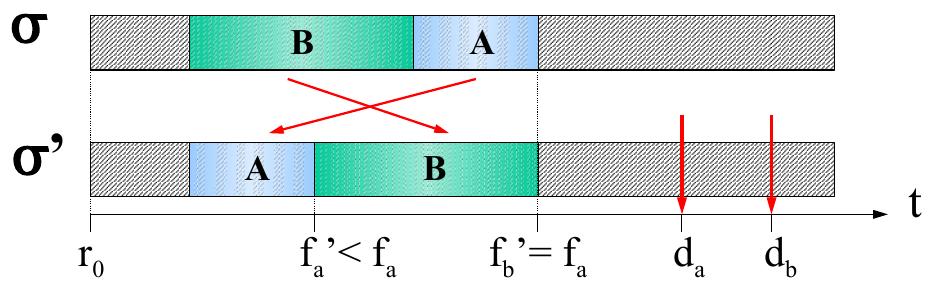
\includegraphics[width=\textwidth]{img/edd_opt}
    \end{minipage}
    \begin{minipage}[t]{0.45\textwidth}
        \centering
        $L_{max} = L_a = f_a - d_a$ \\ 
        $L'_{max}(\sigma') < L_{max}(\sigma)$
        \begin{math}
            \begin{cases}
                L'_a = f'_a - d_a < f_a - d_a \\
                L'_b = f'_b - d_b = f_a - d_b < f_a - d_a
            \end{cases}
        \end{math}
    \end{minipage}
\end{figure}
\\
Siccome $\sigma'$ è equivalente ad EDD solo fino all'istante di tempo $f_a = f'_b$ per poter iterare fino ``all'infinito' è necessario andare a considerare uno scheduler $\sigma \in \{\sigma', \sigma'', ..., \sigma^*\}$. Iterando il ragionamento del confronto fatto per uno scheduler $\sigma$ e $\sigma'$ con tutto l'insieme degli scheduler, in questo modo avremo che: $L_{max}(\sigma') \geq L_{max}(\sigma'') \geq ... \geq L_{max}(\sigma^*)$ andiamo a dimostrare che $\sigma^* = \sigma_{EDD}$ dove $L_{max}(\sigma_{EDD})$ è il minimo valore ottenibile da ogni algoritmo di scheduler. \\
Un \textit{task set} $\mathcal{T}$ è \textbf{fattibile} se $\forall i \; f_i \leq d_i$ quindi avremo che il \textit{finish time del task} è pari a $f_i = \sum_{k = 1}^i C_k$ ma quindi avremo il vincolo che $\forall i \sum_{k = 1}^i C_k \leq D_i$ ovvero che il \textbf{WCET} ovvero l'\textit{worst case execution time} per ogni task sia minore della loro \textit{deadline} assoluta. \\
\textbf{Complessità}:
\begin{itemize}
    \item per ordinare il \textit{task set} $\mathcal{O}(n \log n)$
    \item per garantire l'intero \textit{task set} $\mathcal{O}(n)$
\end{itemize}

\newpage
\section{Earliest Deadline First}
Seleziona il task da eseguire considerando la \textit{deadline} \textbf{assoluta} più imminente.
\begin{itemize}
    \item i task possono arrivare in qualunque istante di tempo $t_i$.
    \item priorità \textbf{dinamiche}.
    \item \textit{fully preemptive tasks}.
    \item minimizza la \textit{lateness} $L_{max}$ massima.
\end{itemize}
\begin{figure}[h]
    \centering
    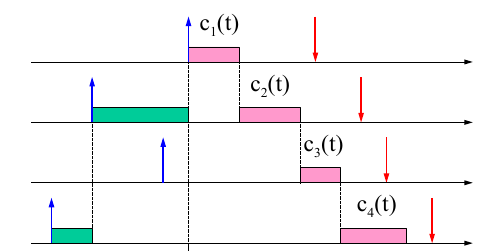
\includegraphics[width=0.5\textwidth]{img/edf_1}
\end{figure}
EDF garantisce la fattibilità della schedulabilità se $\forall i \; \sum_{k = 1}^i c_k(t) \leq d_i - t$. \\
\textbf{Complessità}:
\begin{itemize}
    \item per inserire un nuovo task all'interno del \textit{task set} il \textit{task set} $\mathcal{O}(n)$
    \item per garantire un nuovo task $\mathcal{O}(n)$
\end{itemize}
